\chapter{\protect Introduction}
\label{introduction}

According to Hindu cosmological mythology, ancient people believe that a giant turtle bears the world on its back. Even after we stepped onto the moon at 1969, there are still plenty that we cannot explain. In the novel Lord of the Rings, the author named the path between hobbits as Mordor, which is also the name of the dark area on Pluto$'�$�s moon, Charon. Recently, Mission New Horizons retrieved valuable data about Charon and Pluto. This thesis aimed to investigate the chemistry of VUV and EUV irradiations on CH$_4$+NH$_3$ ice mixtures, which is possibly the main compositions to form the red polar cap on Charon.

\begin{figure}
\centering
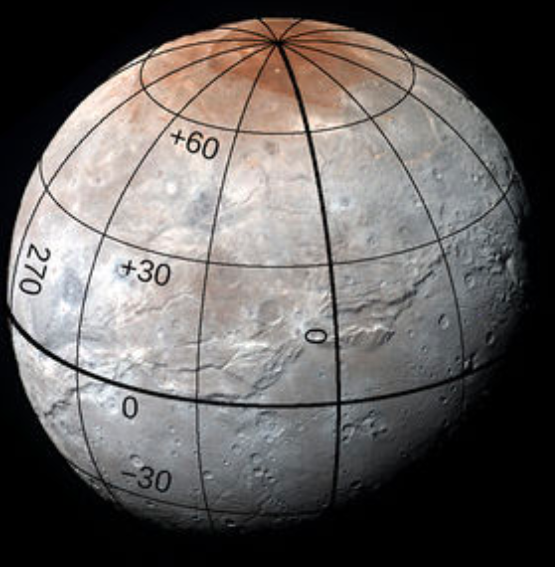
\includegraphics[width=0.5\textwidth]{figures/chapter1/charon.png}
\caption{An overlapped figure of Charon taken from 3 filters of MVIC camera and LORRI camera to show topological details. (quoted from \cite{grundy2016formation})
\label{fig:charon}
\end{figure}

\begin{figure}
\centering
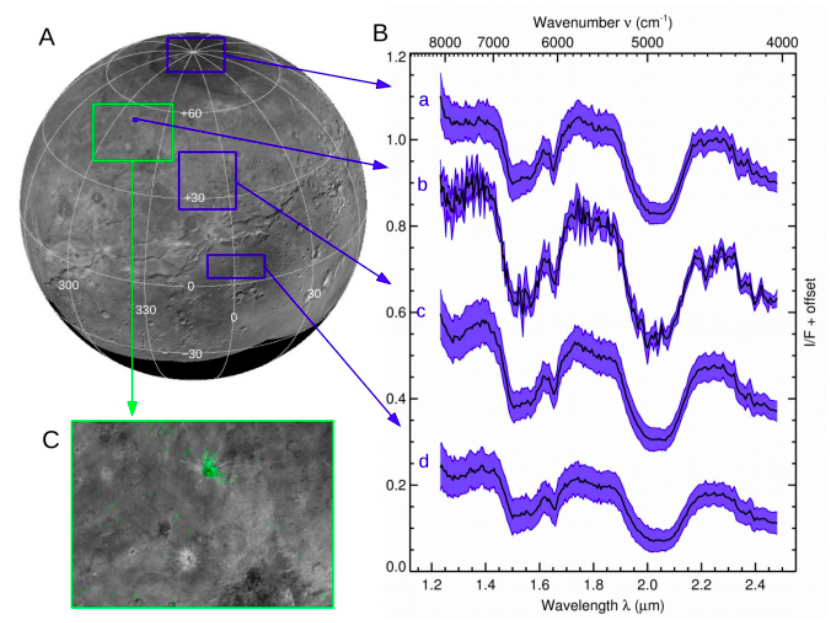
\includegraphics[width=\textwidth]{figures/chapter1/IR.png}
\caption{The 2.2$\um$m absorption taken by LEISA camera colored as green on the topology shown by LORRI camera (A) and the spectra at 4 positions with b taken near organa crater.(quoted from \cite{grundy2016surface})
\label{fig:Charon_IR}
\end{figure}

\begin{figure}
\centering
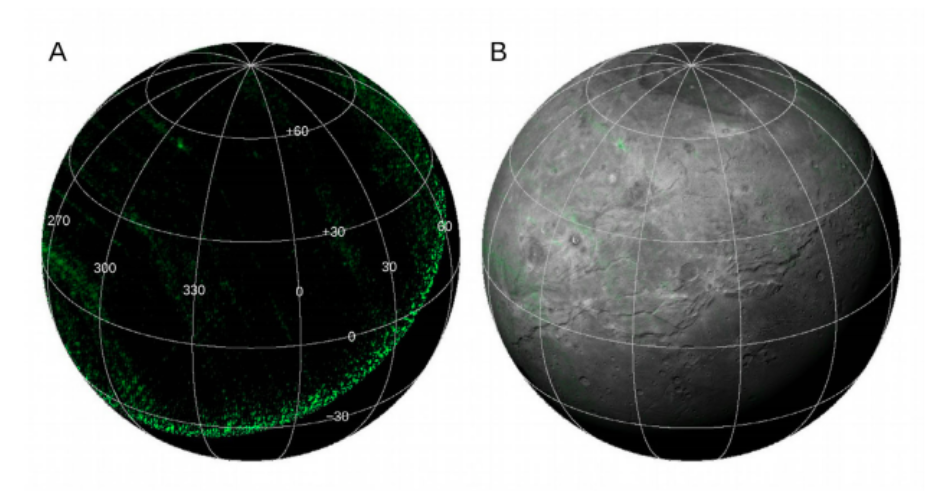
\includegraphics[width=\textwidth]{figures/chapter1/ammonia.png}
\caption{ The 2.2 $\mu$ m absorption taken by LEISA camera with ammonia marked as green (A) and the topology shown by LORRI camera (B).(quoted from \cite{grundy2016surface})
\label{fig:Charon_ammonia}
\end{figure}

\begin{figure}
\centering
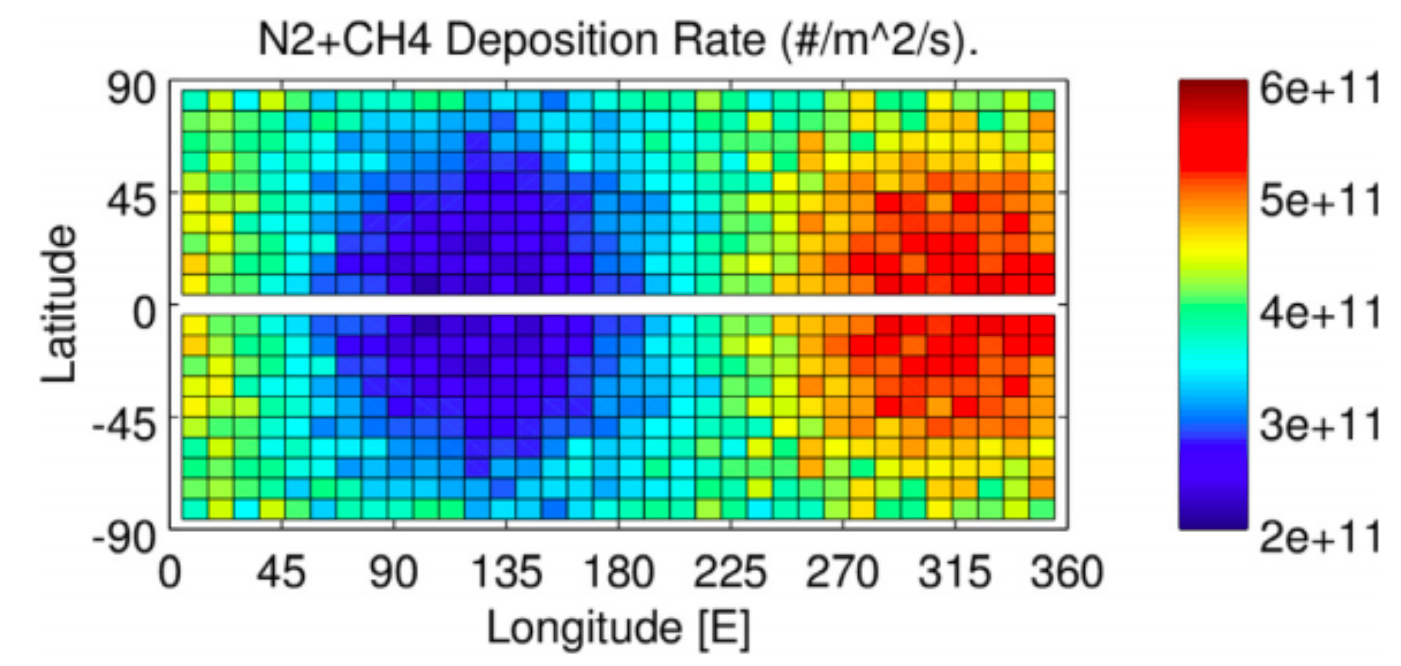
\includegraphics[width=\textwidth]{figures/chapter1/methane.png}
\caption{The simulation of N$_2$ and CH$_4$ model assuming all arrived molecules will stick onto the surface of Charon. Among the deposition rate, 98 \% of them are CH$_4$ because CH$_4$ is lighter and preferentially escapes. The molar fraction of CH$_4$ increase from hypothesized 0.44 \% to 42 \% in the exobase of Pluto.(quoted from \cite{hoey2017rarefied})
\label{fig:Charon_distribution}
\end{figure}

According to Infrared (IR) spectroscopy, surface of Charon is a mixture of 90 \% H$_2$O and 10 \% tholin at millimetre depth. The main component which forms the dark red cap (tholin) is cold-trapped methane from Pluto$'$��s atmosphere ejecta \cite{hoey2017rarefied}. The second possible component is ammonia. Since ammonia hydrate can be observed by earth-based telescopes \cite{cook2007near}. Also in far IR spectrum taken by LEISA camera on the New Horizons, concentrated ammonia is found on Organa crater (figure \ref{fig:Charon_IR}) and throughout Charon (figure \ref{fig:Charon_ammonia}) \cite{grundy2016surface}. The third component is methane. The presence of nitrogen and other ejecta from Pluto are neglected in this thesis because according to the model of Hoey et al.\cite{hoey2017rarefied} (figure \ref{fig:Charon_distribution}), during New horizons$'$ approach, 98 \% of the arrived ejecta is CH$_4$. CH$_4$ remains undetectable by infra-red spectroscopy nor VUV spectroscopy.

Ly-$\alpha$ appears to be the largest source in the dark side of Charon, with attributions from both solar occultation (70 \%) and resonance scattering by atomic hydrogen flow (30 \%) in the solar system at flux $3.5 \times 10^7$ photons cm$^{-2}$ s$^{-1}$ onto the winter pole of Charon \cite{grundy2016formation}. The flux is 50 \% larger than expected before Mission New Horizons \cite{gladstone2015lyalpha}. CH$_4$ deposits at temperature below 25 K at pressure $7.4 \times 10^{-14}$ torr. The time for depositing CH$_4$ is 2 times longer at the pole (130 earth years) than at 45˚ lattitude according to the thermal model of Grundy et al. \cite{grundy2016formation} (figure \ref{fig:Charon_thermal). In order to understand the formation of tholin at different latitudes of Charon, we performed VUV irradiation on CH$_4$+NH$_3$ experiments with different ratios (including 3:2, 1:5, 1:10 and 1:20 for CH$_4$+NH$_3$ to simulate the conditions at different latitudes on Charon with base pressure $3 times 10^{-10}$ torr, simulating atmosphere on Charon at 15 K, which corresponds to temperature on Charon at winter times \cite{grundy2016formation} in interstellar processing system (IPS) \cite{chen2013vacuum}.

\begin{figure}
\centering
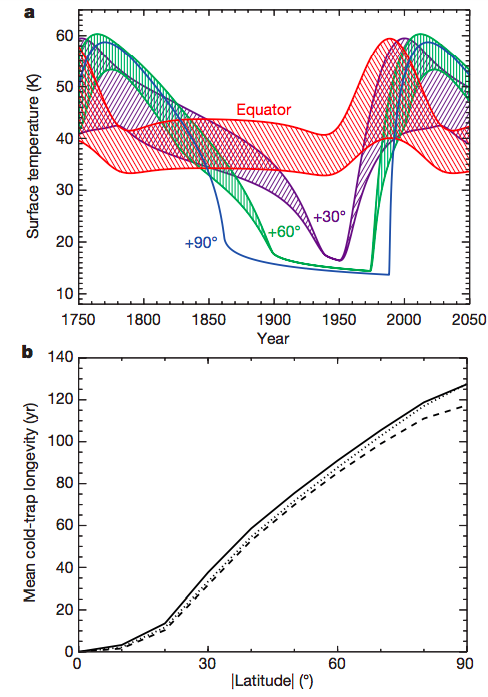
\includegraphics[width=0.5\textwidth]{figures/chapter1/thermal.png}
\caption{The temperature of Charon with thermal inertia 10 J m$^{-2}$ K$^{-1}$ s$^{-1/2}$ in 1750 to 2050 Earth years (a) and longest time the Latitude is under 25 K with the model averaged for 3 Myr with 2.5 (solid) 10 (dotted) and 40 (dashed) J m$^{-2}$ K$^{-1}$ s$^{-1/2}$ (b).(quoted from \cite{grundy2016formation})
\label{fig:Charon_thermal}
\end{figure}

Apart from VUV irradiation, EUV irradiation also took part. VUV irradiation is believed to be the main process to convert CH$_4$ into heavier molecules which remained on the surface of Charon until the temperature of Charon become 60 K, at which methane evaporates from the ice. The ice is then further processed by EUV, solar wind, coronal mass ejections and interstellar pickup ions, etc to produce the tholin on Charon \cite{grundy2016formation}. The EUV irradiation (>12.4 eV) is $8.7 \times 10^7 eV cm^{-2} s^{-1}$ at mean heliocentric distance 39 A.U. whereas VUV irradiation (Ly-$\alpha$) is $1.9 \times 10^9 eV cm^{-2} s^{-1}$. In order to investigate the effectiveness of EUV to VUV irradiation, we kept temperature of CH$_4$+NH$_3$ (3:2 \& 1:5) ice mixtures at 15 K and use the monochromatic 30.4 nm (He II) light provided by High flux beamline at National Synchrotron Radiation Research Centre (NSRRC) in Taiwan to irradiate the ice mixtures.

In this text, we will introduce the formation reaction mechanisms of CH$_4$+NH$_3$ ice mixtures in EUV and VUV irradiation, effectivness with electron irradiation experiments and a functional group comparison with tholin on Titan will be made. With these results, we will have a better understanding about Charon and some astrophysical implications will be presented in chapter \ref{astron}.
